 \documentclass[%
USenglish,%
pdftex,%
compress,%
10pt,%
svgnames%
,handout
]
{beamer}

\usefonttheme[onlymath]{serif}
\usepackage[ansinew]{inputenc}      % direkte Eingabe von Umlauten
%\usepackage{times}   % uses times, helvetica and courier
%\usepackage{mathptm}   % uses times, helvetica and courier
%\usepackage{tabularx}
\usepackage{graphicx}   % picture inclusion
%\usepackage{exscale}
\usepackage{amsmath}    % extended math stuff
\usepackage{amsfonts}   % corresponding fonts
%\usepackage{listings}   % for including code passages
\usepackage{bm}         % improved Greek bold math

\usepackage[square]{natbib}  % reference 
\usepackage{booktabs}
\usepackage{ae}          % PDF-compatible fonts
\usepackage{multimedia}
% \usepackage[pdftex,colorlinks]{hyperref}   % for hyperlinks etc.

\setbeamertemplate{footline}[frame number]
%%----[beamer outer theme]----------------------------------------------------------------------
%\mode<presentation>
%
%\setbeamercolor{section in head/foot}{parent=palette quaternary}
%\setbeamercolor{subsection in head/foot}{parent=palette primary}
%
%\setbeamercolor{author in head/foot}{parent=section in head/foot}
%\setbeamercolor{title in head/foot}{parent=subsection in head/foot}
%
%\usesectionheadtemplate
%  {\hfill\insertsectionhead}
%  {\hfill\color{fg!50!bg}\insertsectionhead}
%
%\defbeamertemplate*{headline}{split theme}
%{%
%  \leavevmode%
%  \begin{beamercolorbox}[wd=.5\paperwidth,ht=2.5ex,dp=1.125ex]{section in head/foot}%
%    \insertsectionnavigationhorizontal{.5\paperwidth}{\hskip0pt plus1filll}{}%
%  \end{beamercolorbox}%
%  \begin{beamercolorbox}[wd=.5\paperwidth,ht=2.5ex,dp=1.125ex]{subsection in head/foot}%
%    \insertsubsectionnavigationhorizontal{.5\paperwidth}{}{\hskip0pt plus1filll}%
%  \end{beamercolorbox}%
%}
%
%\defbeamertemplate*{footline}{split theme}
%{%
% \leavevmode%
% \hbox{\begin{beamercolorbox}[wd=.5\paperwidth,ht=2.5ex,dp=1.125ex,leftskip=.3cm plus1fill,rightskip=.3cm]{author in head/foot}%
%   \usebeamerfont{author in head/foot}\insertshortauthor
% \end{beamercolorbox}%
% \begin{beamercolorbox}[wd=.5\paperwidth,ht=2.5ex,dp=1.125ex,leftskip=.3cm,rightskip=.3cm plus1fil]{title in head/foot}%
%%    \usebeamerfont{title in head/foot}\insertshorttitle
%    \usebeamerfont{title in head/foot}\textbf{\insertshorttitle}\hfill\includegraphics[width=2cm] {../common/cogbotlab.pdf}
% \end{beamercolorbox}}%
% \vskip0pt%
%}
%
%\mode<all>
%%%---------------------------------------------------------------------------------------------
%
%%%----[beamer finetuning, color definitions + TUM CI]----------------------------------------------------------------------
%\usecolortheme{seahorse}
%\definecolor{TUMgreenPrint}{RGB}{162,173,0}
%\definecolor{TUMlightgreen}{RGB}{181,202,130}
%\definecolor{TUMorange}{RGB}{255,128,0}
%\definecolor{TUMlightblue}{RGB}{65,190,255}
%\definecolor{CogBotLightblue}{RGB}{66,128,194}
%\definecolor{CogBotDarkblue}{RGB}{15,71,129}
%\definecolor{CogBotRed}{RGB}{192,38,45}
%\definecolor{CogBotLightest}{RGB}{219,248,223}
%\setbeamercolor{titlelike}{fg=CogBotRed,bg=}
%\setbeamerfont{titlelike}{size=\large}
%%\usecolortheme[cmyk={0.9,0.48,0.0,0.0}]{structure}  % Pantone 285 C
%\usecolortheme[named=CogBotDarkblue]{structure}  % Pantone 285 C
%
%\beamertemplatenavigationsymbolsempty
%%%\beamertemplateshadingbackground{blue!15}{blue!0}
%\setbeamercolor{fig}{fg=black,bg=gray!30}
%\setbeamercolor{block title}{fg=white,bg=CogBotLightblue}
%\setbeamercolor{block body}{fg=black,bg=white}
%\setbeamercolor{proof}{fg=black,bg=TUMorange}
%\setbeamercolor{def}{fg=black,bg=TUMlightgreen}
%\beamerboxesdeclarecolorscheme{def}{CogBotDarkblue}{white}
%\beamerboxesdeclarecolorscheme{proof}{CogBotRed}{white}
%\beamerboxesdeclarecolorscheme{str}{CogBotLightlue}{white}
%\setbeamercovered{dynamic}
%\beamertemplateballitem
%%\beamertemplatenumberedballsectiontoc
%\beamertemplateshadingbackground{gray!8}{gray!8}
%\setbeamertemplate{blocks}[rounded][shadow=true]
%%\useinnertheme[shadow]{rounded}
%%%---------------------------------------------------------------------------------------------

%%----[prettier graphics inclusion (optional)]----------------------------------------------------------------------

\newcommand{\imgcrop}[4]{  % filename, title, boxwidth, viewport
    \centering\begin{beamerboxesrounded}[upper=fig,lower=block body,width=#3,shadow=true]{#2}
        \includegraphics[width=\textwidth,viewport=#4]{pics/#1}
    \end{beamerboxesrounded}
}
\newcommand{\imgbox}[3]{   % filename, title, boxwidth
    \centering\begin{beamerboxesrounded}[upper=fig,lower=block body,width=#3,shadow=true]{#2}
        \includegraphics[width=\textwidth]{pics/#1}
    \end{beamerboxesrounded}
}
%
%
%
%
\begin{document}
% =====================================================================
% \hypersetup{pdftitle={Baxter Anomaly Data Set}}

\title{The Baxter Anomaly Data Set}
\author{Marvin Ludersdorfer}
\institute{Technische Universit\"{a}t M\"{u}nchen}

\date{}

\frame{\titlepage}
%%
\begin{frame}
	\frametitle{Motivation}
    \begin{figure}
        \centering
        \includegraphics[width=\textwidth]{figs/robots}
    \end{figure}
    
    \vfill
    \begin{block}{Assumptions}
        \begin{itemize}
            \item motion is important part of any (robot) task
            \item anomaly in robot motion corresponds to change in dynamic behavior
        \end{itemize}
        $\Rightarrow$ model anomalies as changes in robot control parameters
	\end{block}
\end{frame}

\begin{frame}
	\frametitle{Experiment}
	\begin{columns}[onlytextwidth]
        \begin{column}{.5\textwidth}
        \begin{block}{`normal' trial}
            \rule{.9\columnwidth}{3cm}
            %\movie[width=\columnwidth,height=.75\columnwidth,poster,loop]{}{movs/DSC5992.mp4}
        \end{block}
        \end{column}
        \begin{column}{.5\textwidth}
        \begin{block}{anomalous trial}
            \rule{.9\columnwidth}{3cm}
            %\movie[width=.99\columnwidth,height=.74\columnwidth,poster,loop]{}{movs/DSC5992.mp4}
        \end{block}
        \end{column}
    \end{columns}
    TODO: record videos of one normal and one anomalous trial
\end{frame}

\newcommand{\info}[1]{{\footnotesize\textcolor{gray}{#1}}}
\newcommand{\unit}[2]{\ensuremath{#1\,\mathrm{#2}}}

\begin{frame}
	\frametitle{Data recorded}
    \begin{columns}[onlytextwidth]
        \begin{column}{.6\textwidth}
            \begin{itemize}
                \item measured wrist acceleration \info{@ \unit{25}{Hz}}
                \item commanded configuration \info{as it happens}
                \item measured configuration \info{@ \unit{96}{Hz}}
                \item generated torques \info{@ \unit{149}{Hz}}
                \item commanded torques \info{@ \unit{96}{Hz}}
                \item measured torques \info{@ \unit{96}{Hz}}
                \item camera images \info{$320\times 200$ pixels @ \unit{25}{Hz}}
            \end{itemize}
        \end{column}
        \begin{column}{.4\textwidth}
            \begin{figure}
                \centering
                \includegraphics[width=.9\columnwidth]{figs/baxterjoints}
            \end{figure}
        \end{column}
    \end{columns}
\end{frame}

\begin{frame}
	\frametitle{Data set structure}
    \begin{columns}[onlytextwidth]
        \begin{column}{.6\textwidth}
            Two data sets
            \begin{itemize}
                \item `normal' \texttt{201508061628without.h5}
                \item anomalous \texttt{201508071533with.h5}
            \end{itemize}
            contain each
            \begin{itemize}
                \item trials $0, \ldots, 99$
            \end{itemize}
            where each trial contains
            \begin{itemize}
                \item acceleration
                \item configuration
                \item effort
                \item images
            \end{itemize}
            which in turn hold the mentioned data fields
        \end{column}
        \begin{column}{.4\textwidth}
            \begin{figure}
                \centering
                \includegraphics[width=.7\columnwidth]{figs/h5}
            \end{figure}
        \end{column}
    \end{columns}
\end{frame}

\newcommand{\datawidth}{.43\textwidth}
\begin{frame}
	\frametitle{Looking at data: `Normal' data}
	\begin{figure}
        \centering
        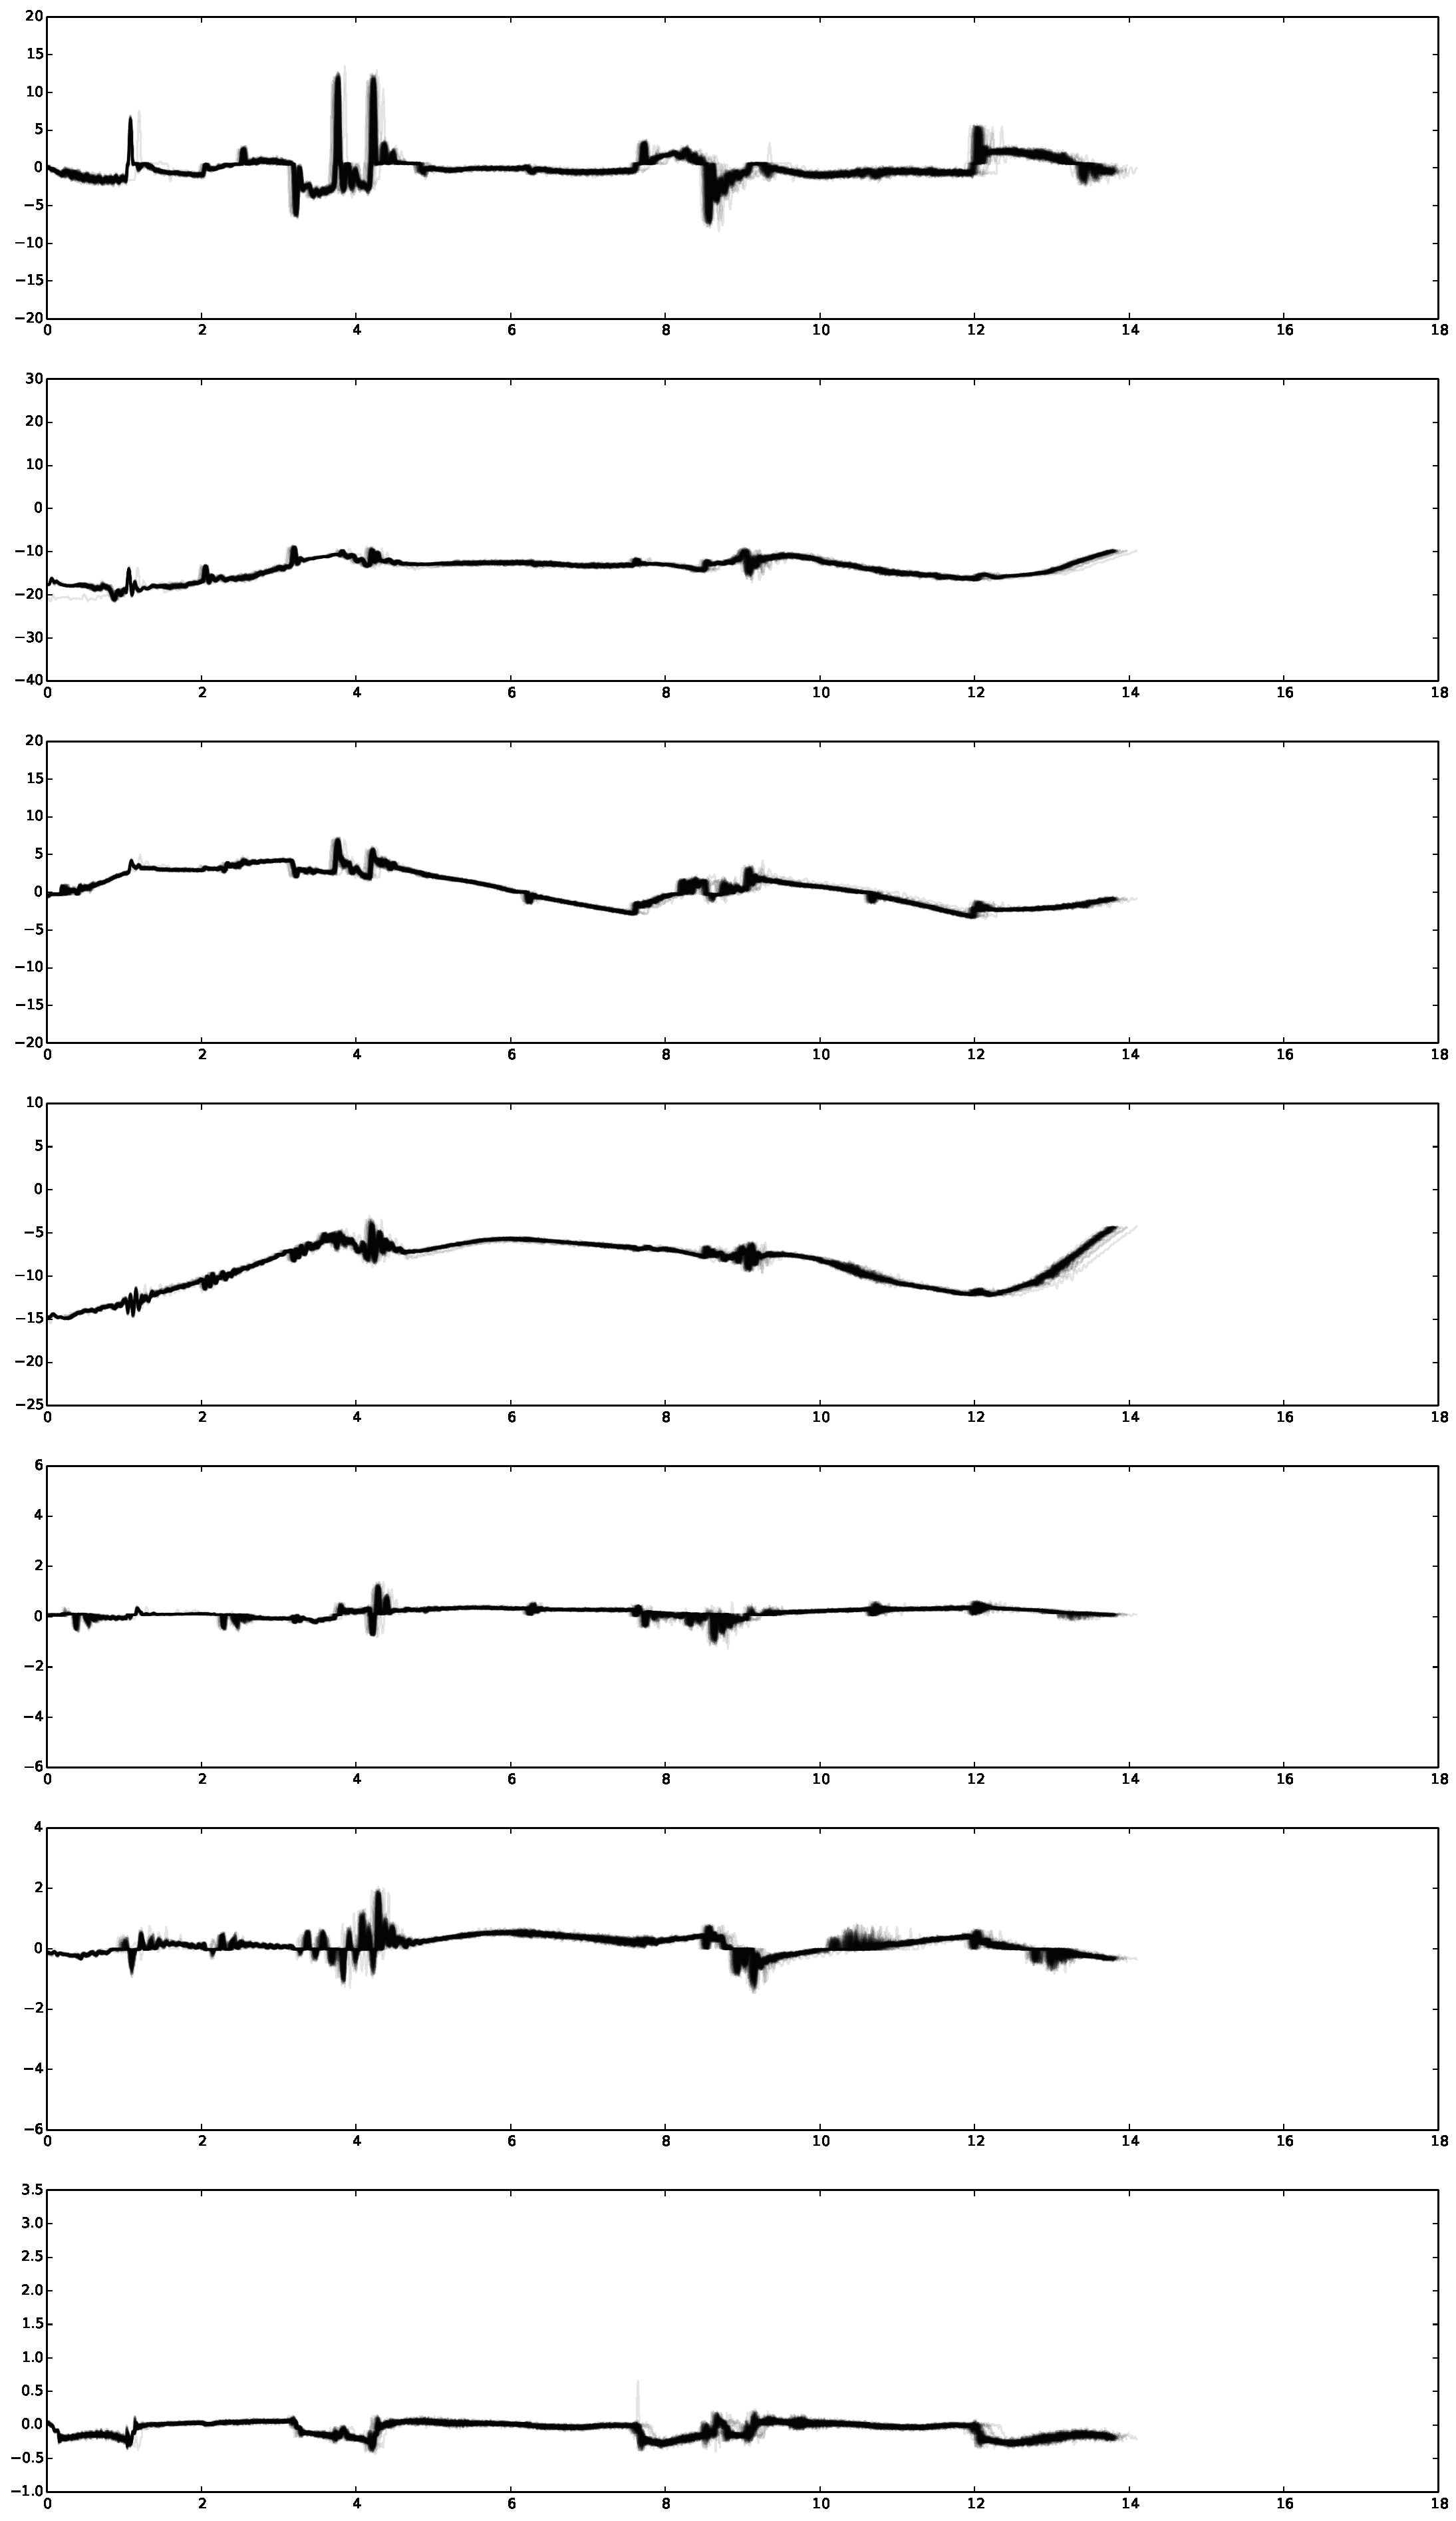
\includegraphics[width=\datawidth]{figs/no_anomaly3.png}
    \end{figure}
\end{frame}

\begin{frame}
    \frametitle{Looking at data: Anomalous data}
    \begin{figure}
        \centering
        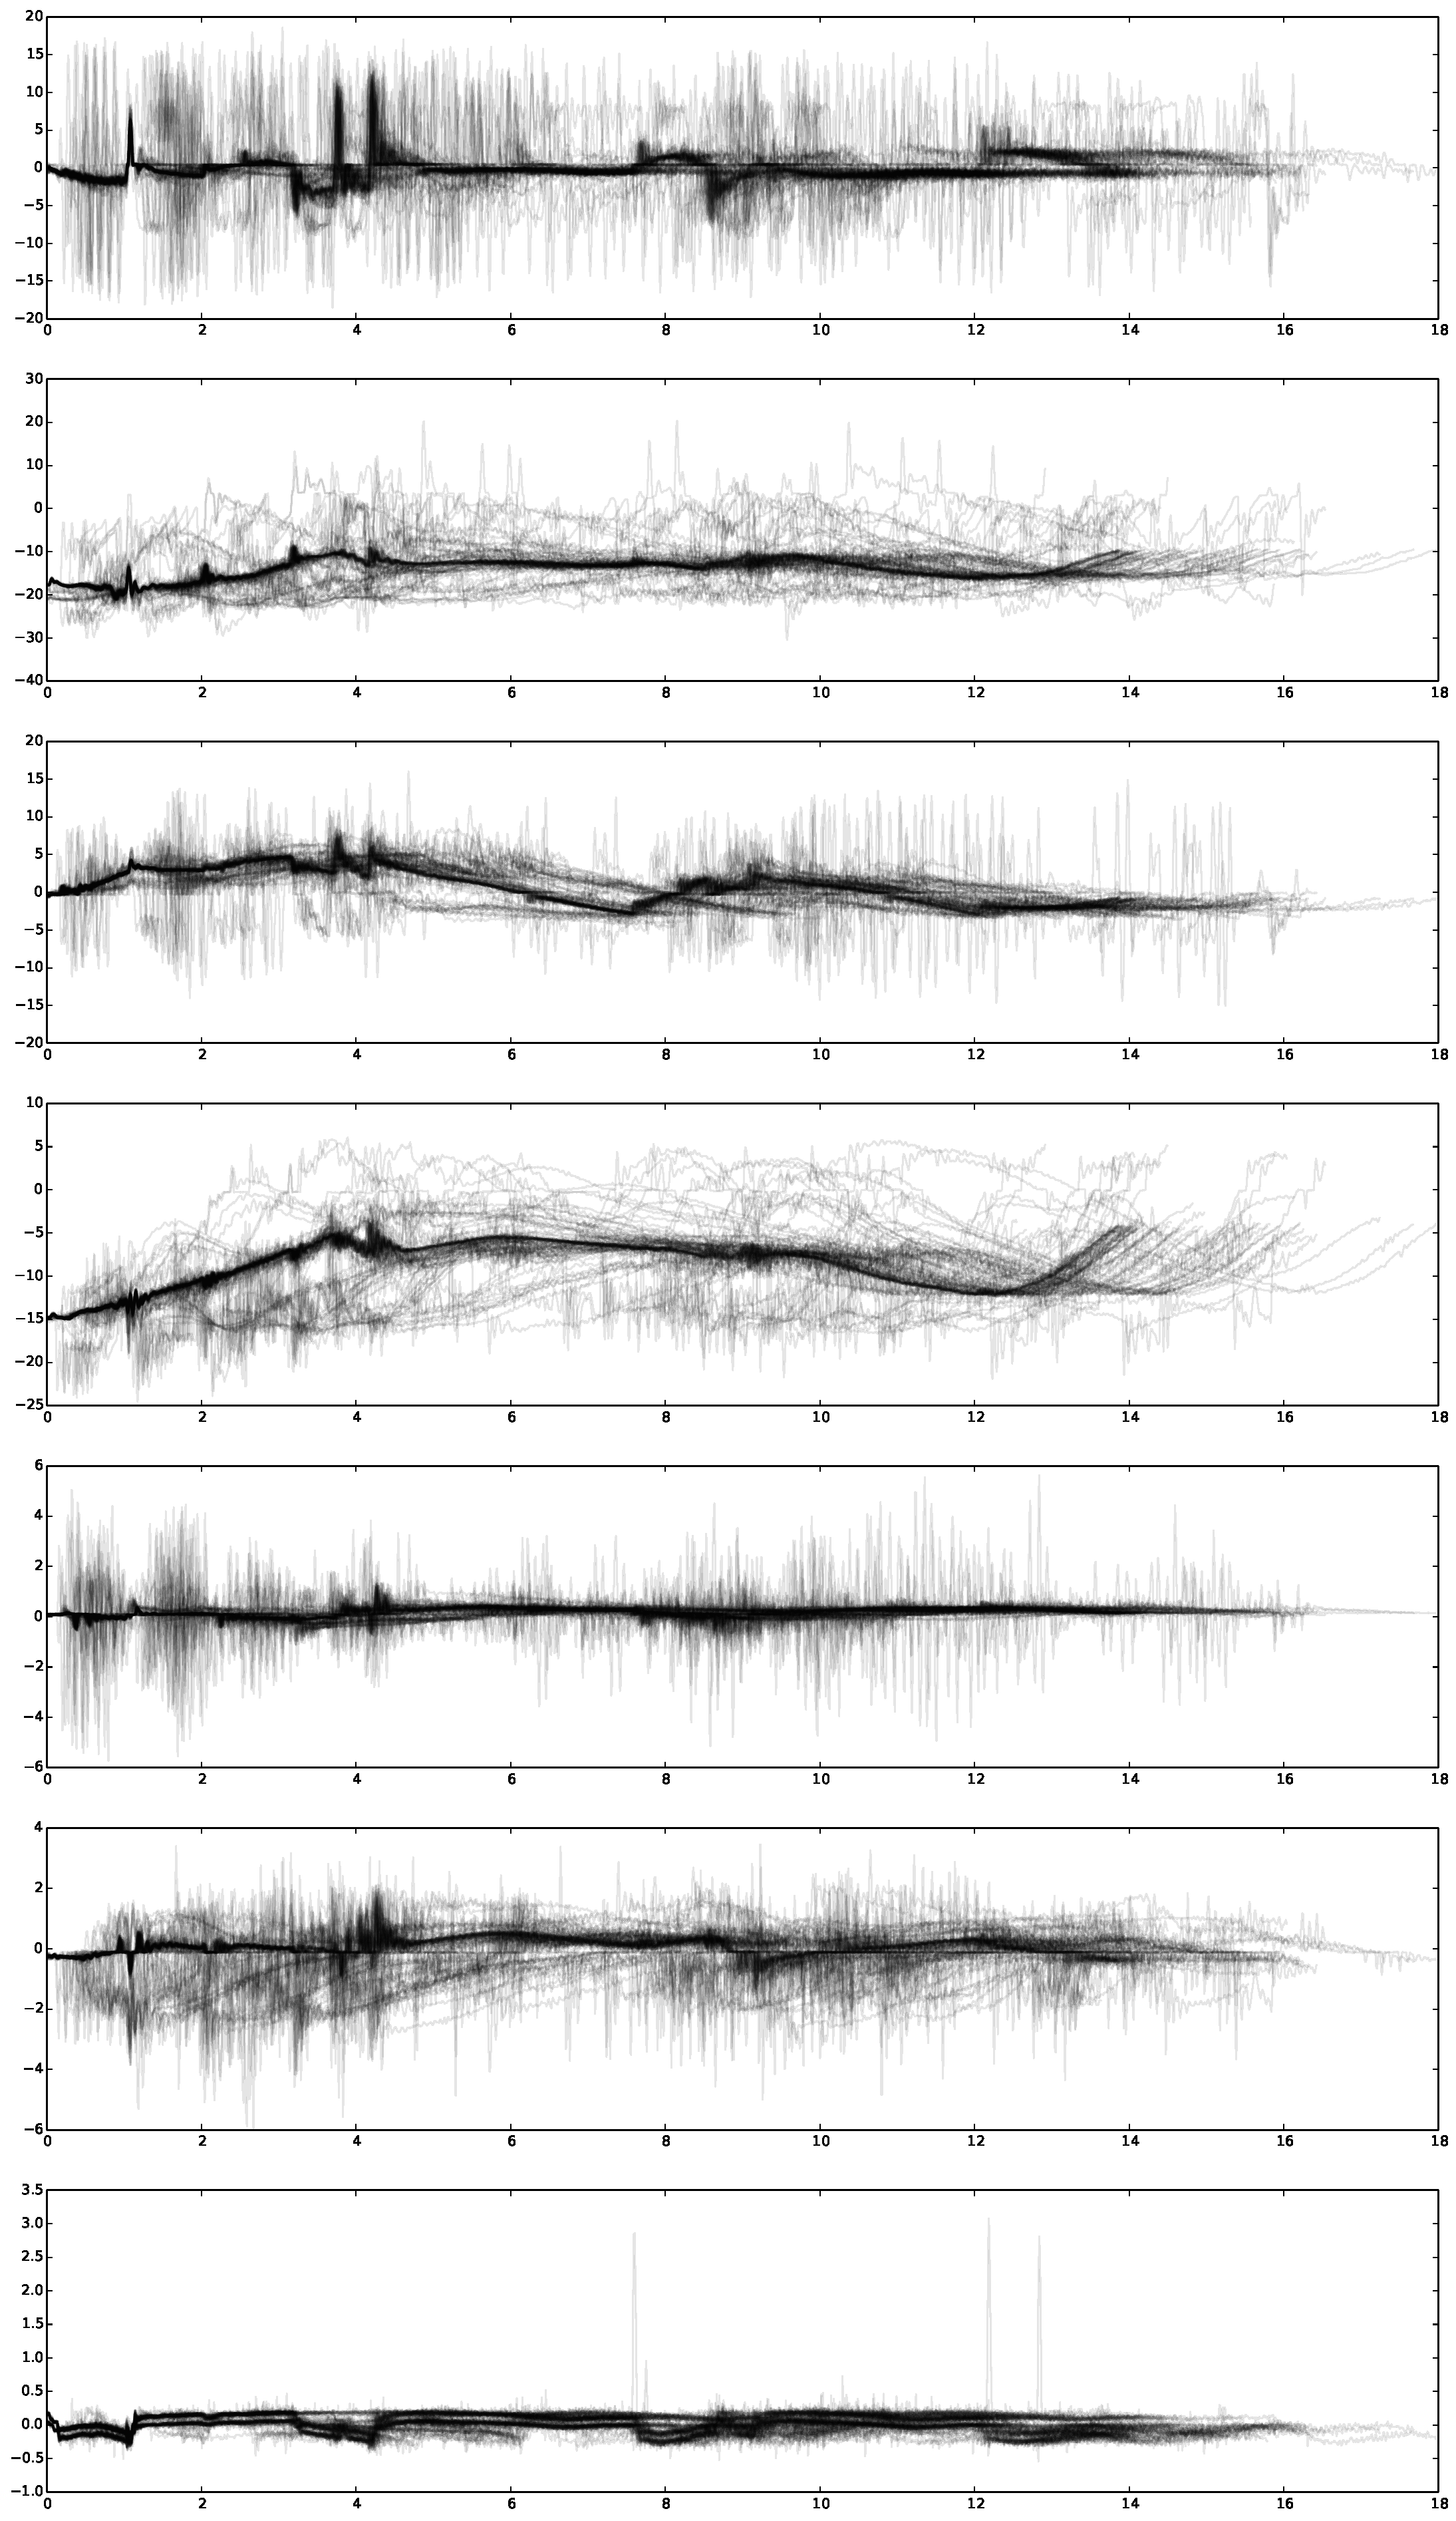
\includegraphics[width=\datawidth]{figs/controller_broke3.png}
    \end{figure}
\end{frame}

\begin{frame}
    \frametitle{Looking at data: Close-up anomaly data (1)}
    \begin{figure}
        \centering
        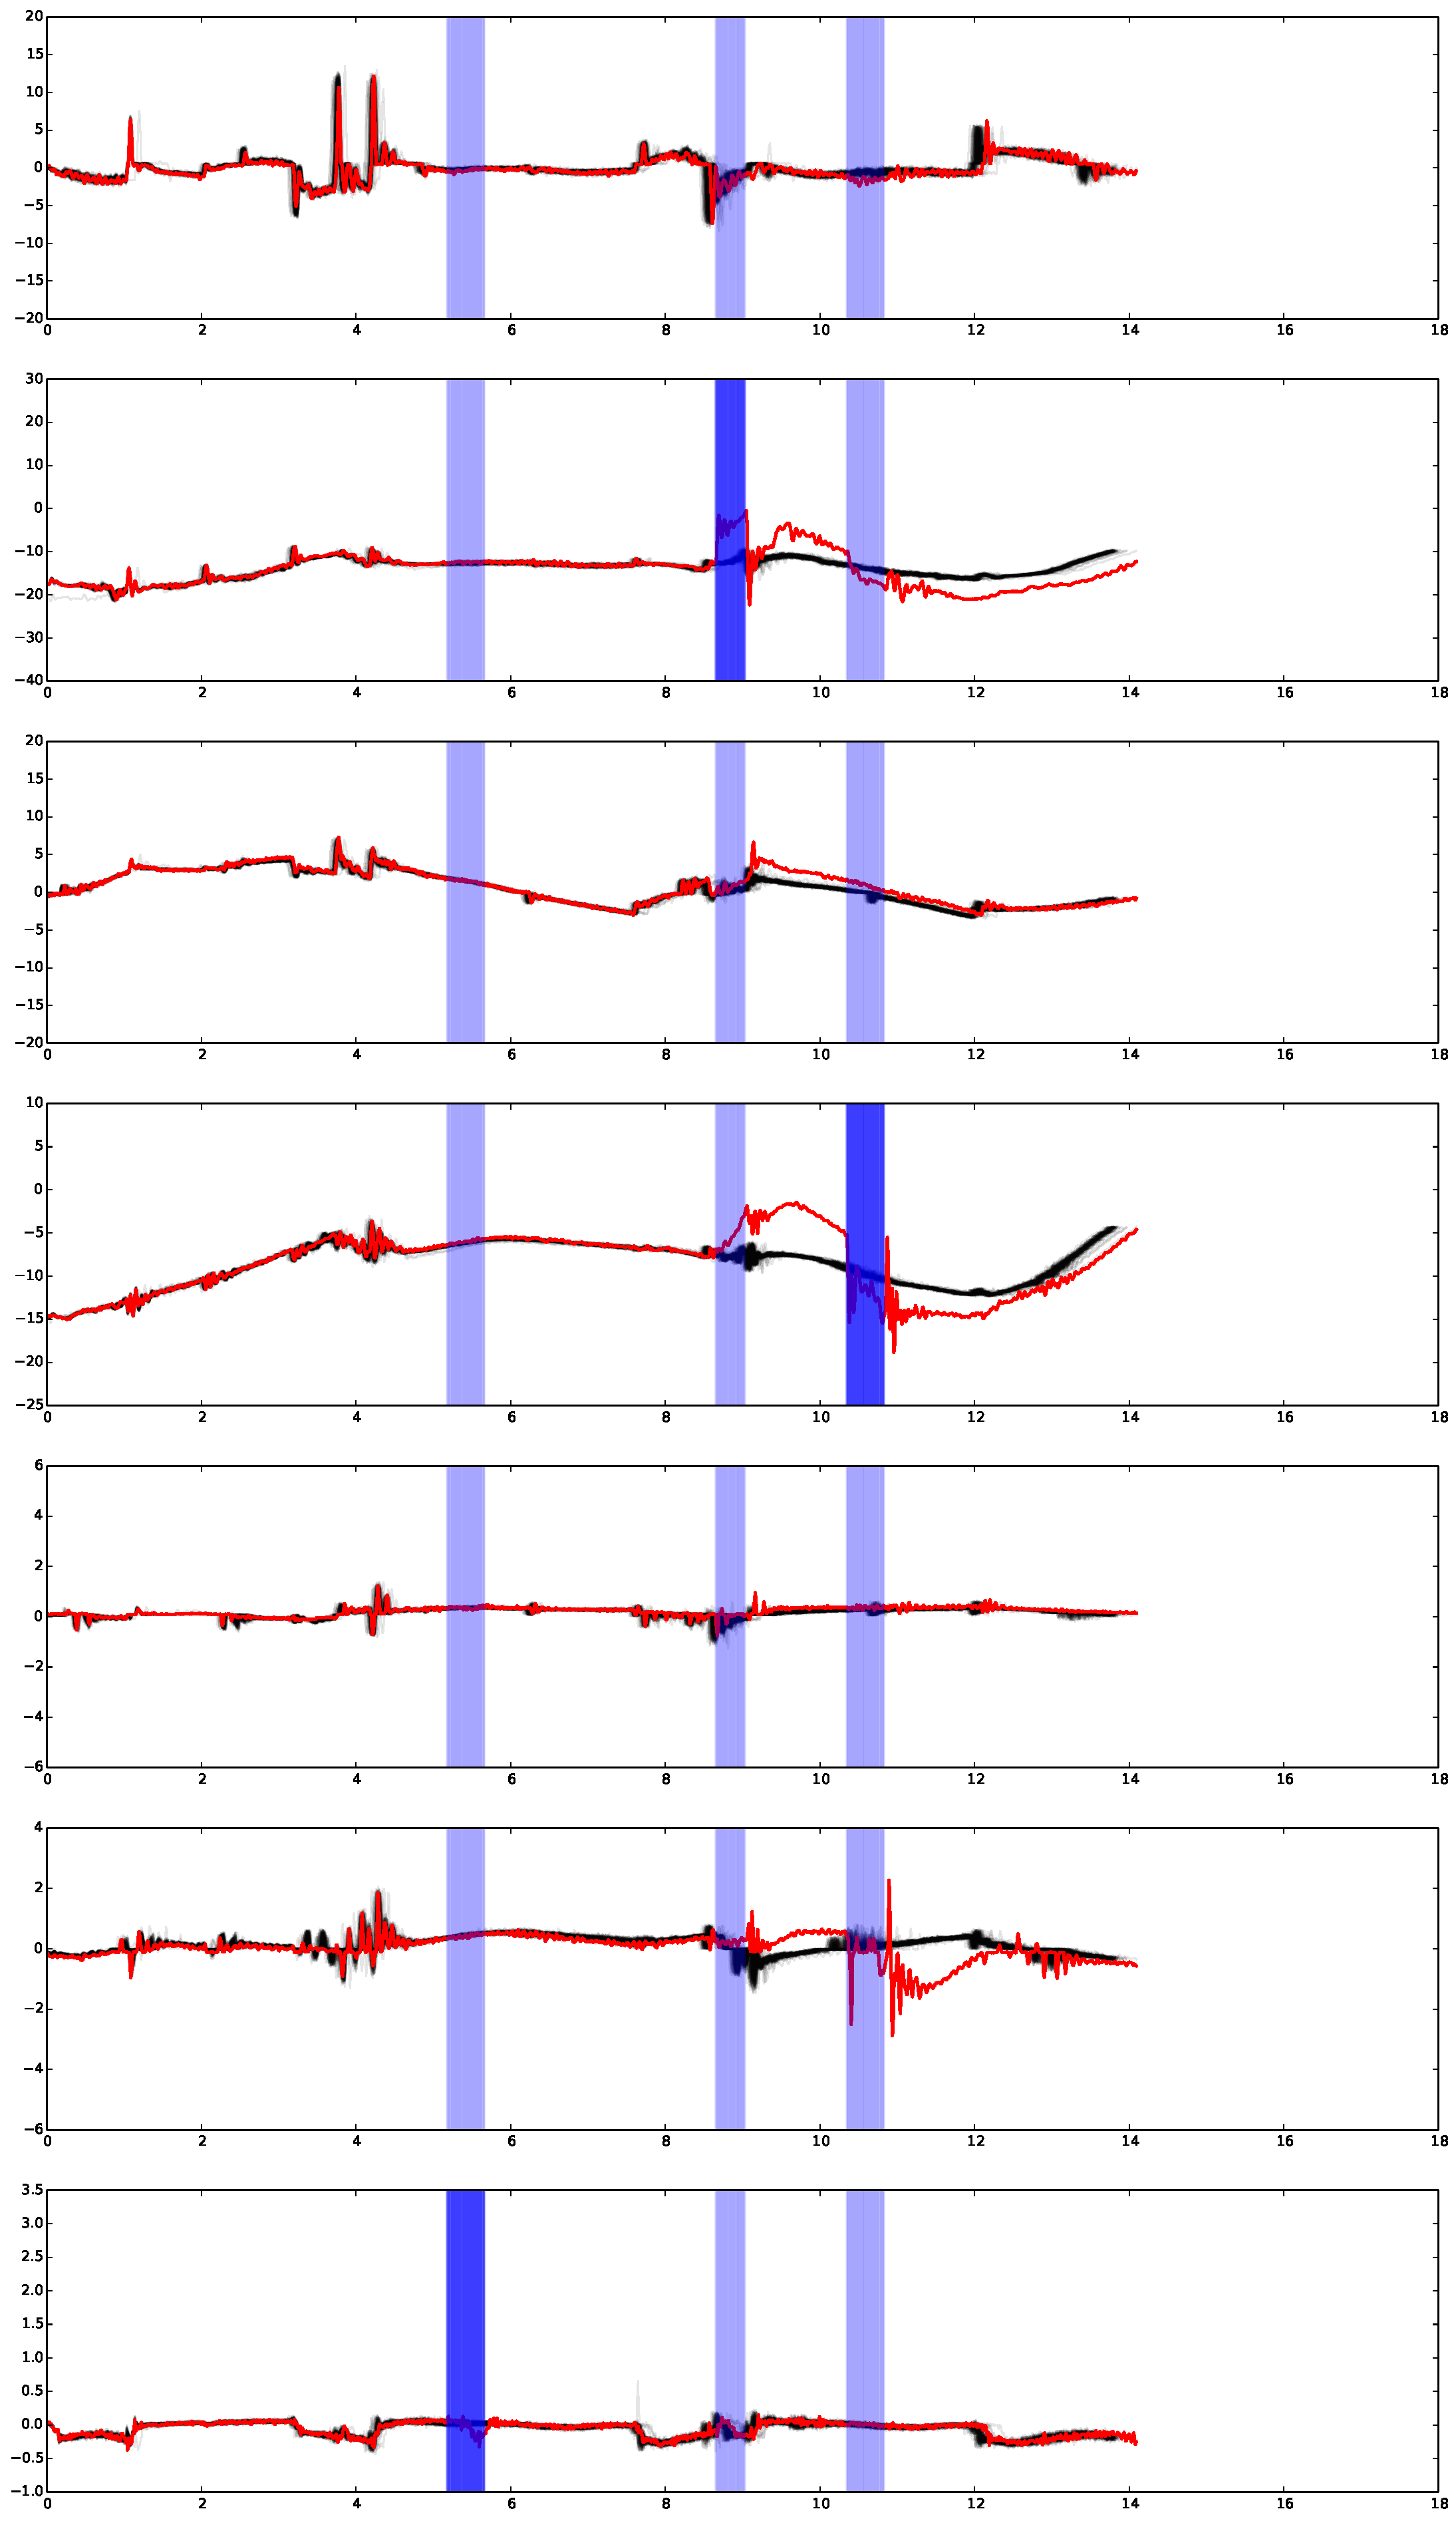
\includegraphics[width=\datawidth]{figs/anomaly12.png}
    \end{figure}
\end{frame}

\begin{frame}
    \frametitle{Looking at data: Close-up anomaly data (2)}
    \begin{figure}
        \centering
        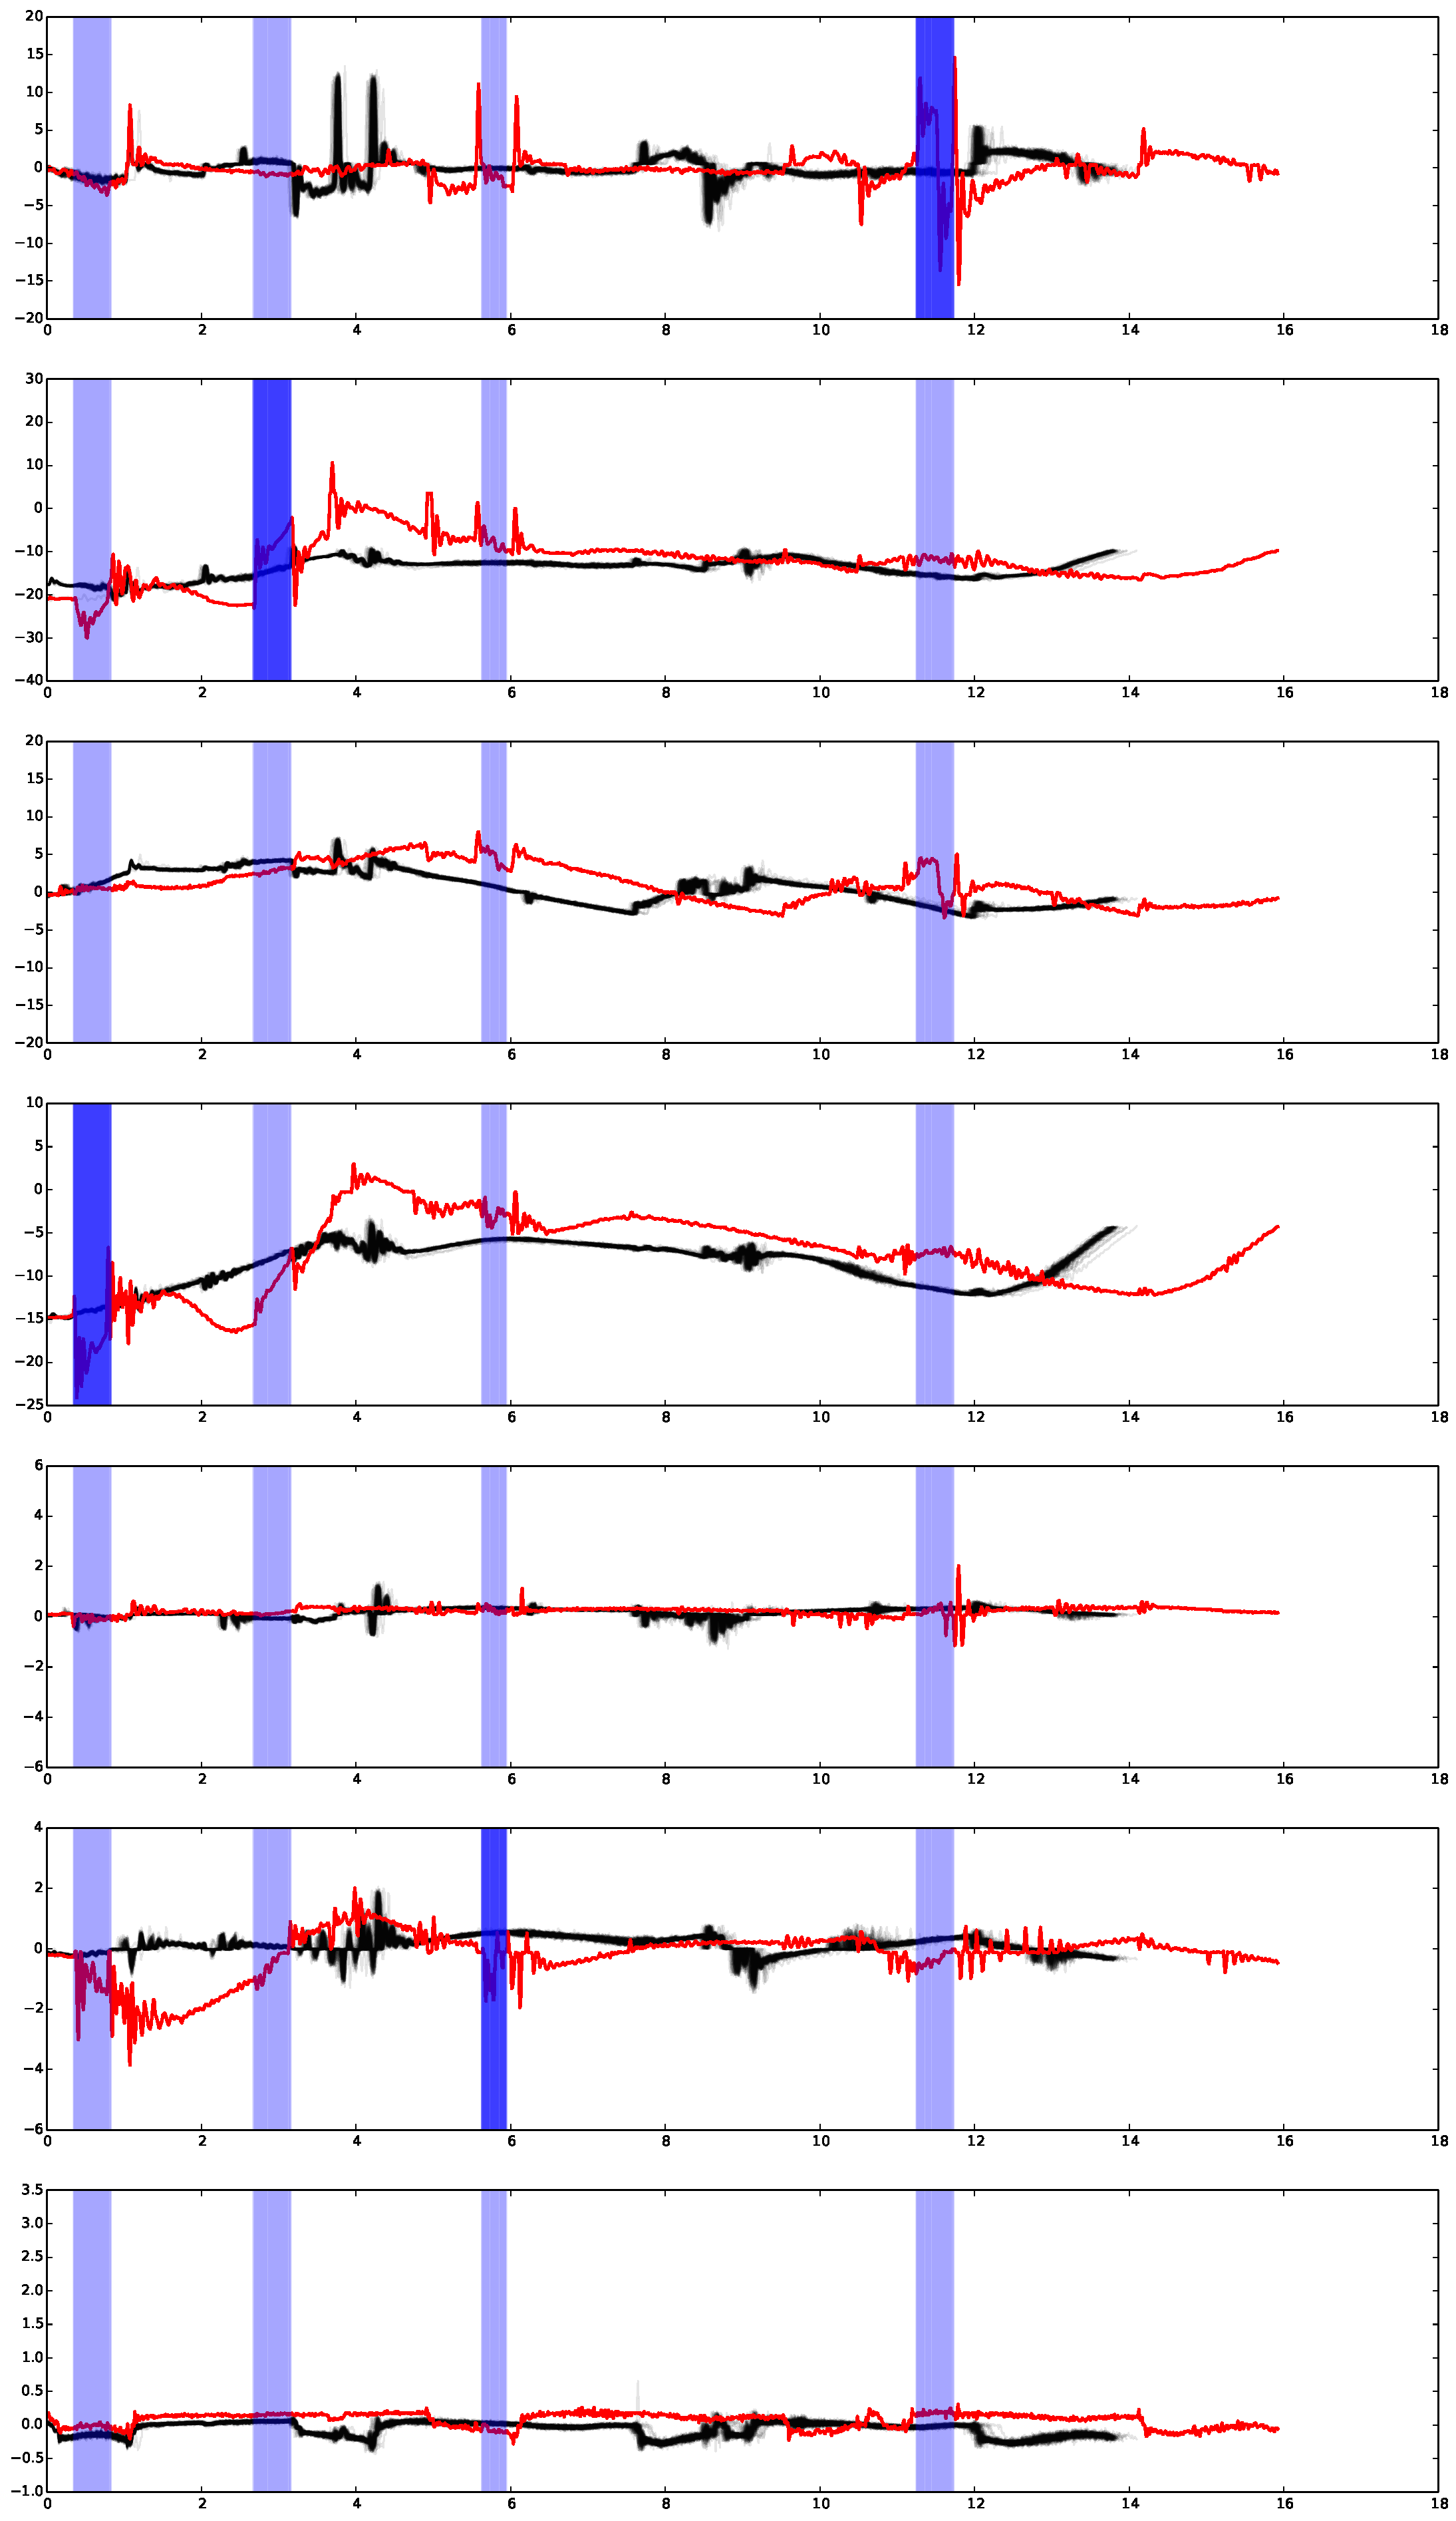
\includegraphics[width=\datawidth]{figs/anomaly50.png}
    \end{figure}
\end{frame}

\begin{frame}
    \frametitle{Where to get the data?}
    Go to \url{https://www.brml.tum.de/BaxterCollision}
    and log on with
    \begin{itemize}
        \item user: \texttt{AnomalyWeb@brml.tum.de}
        \item pwd: \texttt{hit\_Baxter01}
    \end{itemize}
    \vspace{1cm}
    The data we were looking at today is in
    \begin{itemize}
        \item `normal': \texttt{data/preliminary\_control/no\_anomaly\_3}
        \item anomalous: \texttt{data/preliminary\_control/controller\_broke\_3}
        \item plots: \texttt{data/preliminary\_control/Anomaly data nosing-no\_anomaly\_3\_+\_controller\_broke\_3.ipynb} 
    \end{itemize}
    
\end{frame}

\end{document}
